\chapter{Afstæðiskenningin}


\begin{tcolorbox}

\iduck{The views of space and time which I wish to lay before you have sprung from the soil of experimental physics, and therein lies their strength. They are radical. Henceforth, space by itself, and time by itself, are doomed to fade away into mere shadows, and only a kind of union of the two will preserve an independent reality.} \\

\vspace{-0.5cm}
\raggedleft{- \textbf{Hermann Minkowski, 1908}}
\end{tcolorbox}

\section{Inngangur}

Það eru tvær afstæðiskenningar kenndar við Einstein. Annars vegar takmarkaða afstæðiskenningin og hinsvegar almenna afstæðiskenningin. Sú fyrri, takmarkaða afstæðiskenningin, er í rauninni frekar einföld kenning hvað stærðfræðina varðar og Einstein eyddi sjálfur miklu púðri í að setja kenninguna fram þannig að almúgamaðurinn gæti skilið hana. Hinsvegar eru niðurstöður hennar gjarnan í mótsögn við forhugmyndir fólks um það hvernig heimurinn virkar. Hún er líka gegnumsýrð af svokölluðum þversögnum (sem reynast síðan aldrei vera í mótsögn við kenninguna). Það sem vefst sér í lagi fyrir fólki er sú hugmynd að tími og rúm séu á sama tíma samtvinnuð og afstæð hugtök. Í takmörkuðu afstæðiskenningunni erum við helst að fjalla um tvö viðmiðunarkerfi $S$ og $S'$ sem eru á afstæðri hreyfingu með hraða $v$ miðað við hvert annað. \\

\setcounter{theorem}{1}

\begin{tcolorbox}
\begin{minipage}{\linewidth}

\begin{wrapfigure}{r}{2in}
\vspace{-0.5cm}
\hspace{0.5cm}
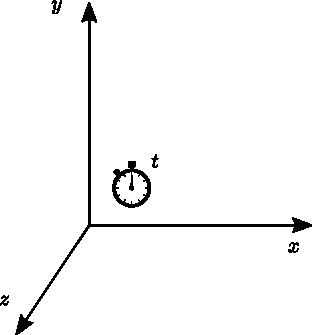
\includegraphics[width = 1.5in]{figures/spacetime.pdf}
\end{wrapfigure}
\textbf{Skilgreining \thetheorem.} Sagt er að \textbf{viðmiðunarkerfi}, $S$, sé fjórvítt hnitakerfi ásamt lengdarkvarða og tímakvarða þar sem að punktarnir í hnitakerfinu eru af gerðinni $(t,x,y,z)$.

\vspace{1.2cm}
\textbf{Atburður}, $A$, er punktur í tímarúminu $A = (t_A,x_A,y_A,z_A)$.
\vspace{1cm}
\end{minipage}
\end{tcolorbox}

Helsti hausverkurinn í takmörkuðu afstæðiskenningunni er að við munum vera með mörg viðmiðunarkerfi í gangi í einu. Það er vegna þess að fólk er svo sjálfhverft og skilgreinir alltaf viðmiðunarkerfið út frá því sem að það sér sjálft! Maður ætti þá að nefna að viðmiðunarkerfið er kyrrt miðað við sjálft sig og ferðast því einungis í jákvæða tímastefnu! Með öðrum orðum þá getum við alltaf litið á sem svo að við séum kyrr í miðju alheimsins en að veröldin snúist um okkur (margir gera þetta nú þegar í annarri merkingu). Við munum þá vera t.d.~með viðmiðunarkerfi $S$ þar sem að athugandi sér atburðinn $A$ gerast í tímarúmspunktinum $A = (t,x,y,z)$. En annar athugandi í viðmiðunarkerfi $S'$ mun sjá sama atburð gerast í $A' = (t',x',y',z')$. Reyndar munum við mestmegnis takmarka okkur við 1+1-vítt tímarúm þ.e.~$(t,x)$. \\

\begin{tcolorbox}
\begin{definition}
Sagt er að \textbf{tregðukerfi} sé viðmiðunarkerfi þar sem tregðulögmál Newtons gildir.
\end{definition}
\end{tcolorbox}

Til þess að reyna að skilja tregðukerfin aðeins betur skulum við byrja á því að skoða myndina hér fyrir neðan:

\begin{figure}[H]
    \centering
    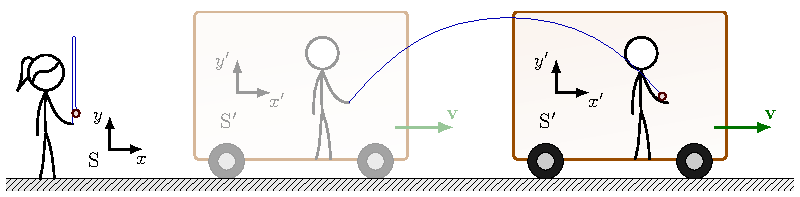
\includegraphics[width=.85\textwidth]{figures/tregdukerfi.pdf}
\end{figure}

Matti og Edda eru í boltaleik. Edda stendur kyrr á jörðinni í viðmiðunarkerfi $S$ og kastar bolta upp í loftið. Matti stendur kyrr í viðmiðunarkerfi $S'$ inni í strætó sem hreyfist með jöfnum hraða $v$ í burtu frá Eddu. Bæði þessi viðmiðunarkerfi eru tregðukerfi\footnote{Tæknilega séð er viðmiðunarkerfi jarðarinnar ekki tregðukerfi því jörðin snýst um sjálfa sig sem veldur því að við sjáum sýndarkrafta eins og t.d.~Coriolis-kraftinn. Við munum hinsvegar til einföldunar hunsa þau áhrif og segja að viðmiðunarkerfi athuganda á jörðinni sé svo gott sem tregðukerfi. Þar að auki er frekar erfitt að keyra strætó með jöfnum hraða svo það er líklegast bara tregðukerfi í stutta stund hverju sinni (viðmiðunarkerfi hættir að vera tregðukerfi ef að það verður fyrir hröðun).}. Skoðum aðeins það sem að Edda sér (sem er það sem myndin sýnir). Edda sér boltann hennar ferðast upp og niður miðað við viðmiðunarkerfið hennar. Hinsvegar, þá sér hún boltann hans Matta ferðast eftir fleygboganum á myndinni því strætóbifreiðin ferðast áfram á meðan að boltinn er í loftinu. En hvað sér Matti í viðmiðunarkerfinu sínu, $S'$? Matti sér boltann sinn fara beint upp og niður (eins og Edda sá boltann sinn). Hann sér síðan boltann hennar Eddu ferðast í fleygboga til vinstri. Við myndum því segja eitthvað eins og að tregðukerfin $S$ og $S'$ eru á afstæðri hreyfingu miðað við hvert annað með hraða $v$. Séð frá Eddu í $S$ þá er það Matti sem að ferðast í burtu frá henni með hraða $v$ til hægri en séð frá Matta í $S'$ þá er alveg eins hægt að segja að það sé Edda sem að ferðast í burtu frá Matta með hraða $v$ til vinstri (eða $-v$ til hægri). Það er því ekki hægt að segja að annað sjónarhornið sé réttara heldur en hitt á meðan að tregðukerfin ferðast með afstæðum hraða miðað við hvert annað. Hinsvegar um leið og strætóbílstjórinn bremsar þá hættir viðmiðunarkerfið hans Matta að vera tregðukerfi og þá fyrst er hægt að færa rök fyrir því að það hafi verið Edda sem var kyrrstæð en ekki Matti! \\

Til þess að reyna að útskýra þetta aðeins betur skulum við líka skoða hvað gerist á myndinni hér fyrir neðan þegar að strætóbílstjórinn eykur hraðann sinn með því að stíga á bensíngjöfina (hann getur líka breytt hraðanum með því að bremsa harkalega). Þá fær strætóvagninn hröðun $a$ til hægri (sem getur verið tímaháð).

\begin{figure}[H]
    \centering
    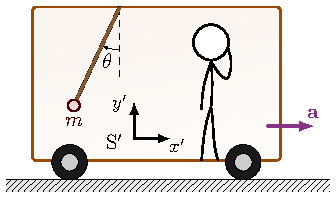
\includegraphics[width=.45\textwidth]{figures/ekkitregdukerfi.pdf}
\end{figure}

Núna er viðmiðunarkerfi Matta, $S'$, ekki lengur tregðukerfi því hann hefur enga útskýringu fyrir því hvers vegna pendúllinn sveigir til vinstri skyndilega. Hann verður því að álykta að hann sé í viðmiðunarkerfi sem finnur fyrir hröðun, það er að segja: hann er ekki í tregðukerfi. \\


\section{Frumsendur afstæðiskenningarinnar}

\begin{tcolorbox}
\begin{theorem}
\textbf{(Frumsendur afstæðiskenningarinnar)}
\begin{enumerate}[label = \textbf{(\arabic*)}]
    \item \textbf{(Afstæðislögmálið)} Lögmál eðlisfræðinnar eru eins í öllum tregðukerfum.
    \item \textbf{(Ljóshraðalögmálið)} Hraði ljóss í tómarúmi er sá sami í öllum tregðukerfum.
\end{enumerate}
\end{theorem}
\end{tcolorbox}

Tæknilega séð er ljóshraðalögmálið innifalið í afstæðislögmálinu en það er mikilvægt að taka það fram því áður fyrr héldu menn að ljósbylgjur bærust í miðli sem þeir kölluðu ljósvakan (e.~\emph{ether}). Til samanburðar við aðrar bylgjur er t.d.~hljóðhraðinn háður hreyfingu hlustanda með tilliti til loftstins og er því ekki sá sami í öllum tregðukerfum. Það er því afar undarlegt að hraði ljóssins sé óháður tregðukerfinu!

\vspace{0.1cm}

Sagan segir að Einstein hafi (þegar hann var 16 ára) áttað sig á seinna lögmálinu með eftirfarandi hugartilraun:

\vspace{0.1cm}

Ímyndum okkur að við höldum á spegli í myrkri og að við ferðumst síðan með ljóshraða. Kveikjum síðan ljósin. Hvað sést þá í speglinum?

\vspace{0.1cm}

Ef hraði ljóssins væri ekki sá sami í öllum tregðukerfum þá myndi ekkert sjást í speglinum. Það er vegna þess að það sem að við sjáum í speglinum er okkar eigið endurvarp. Ljósið þarf að endurkastast af húðinni okkar og lenda síðan á speglinum og ferðast þaðan til baka í augun á okkur. En þessi hugartilraun sýnir að þetta væri í mótsögn við afstæðislögmálið því þar með væru lögmál eðlisfræðinnar ekki eins í öllum tregðukerfum. Þar með væri hægt að nota þessa niðurstöðu til þess að greina með hvaða hraða maður væri að ferðast.

\vspace{0.1cm}

Í því sem eftir kemur þá mun það reynast okkur gagnlegt að hafa skilgreint eftirfarandi fall:


\begin{comment}
\begin{tcolorbox}
\textbf{Hugartilraun Newtons:} Ímyndum okkur að við séum stödd í tregðukerfi með tvær nákvæmlega eins, kyrrstæðar kúlur. Nú gefum við annarri kúlunni snúningshraða um ás sem liggur í gegn um miðju beggja kúlnanna. Þá aflagast kúlan sem snýst örlítið (eins og Jörðin sem er breiðari við miðbaug). Hin kúlan er óbreytt. 
\end{tcolorbox}
\end{comment}

\begin{tcolorbox}
\begin{definition}
Við skilgreinum \textbf{Lorentz-fallið} (líka kallað \textbf{gamma-fallið}) sem fallið:
\begin{align*}
    \gamma(v) = \frac{1}{\sqrt{1 - \left(\frac{v}{c}\right)^2}}
\end{align*}
Það getur líka stundum verið þægilegt að tala um \textbf{beta-fallið}, $\beta = \frac{v}{c}$.
\end{definition}
\end{tcolorbox}

Það er gott að fá myndræna tilfinningu fyrir Lorentz-fallinu:

\begin{figure}[H]
    \centering
    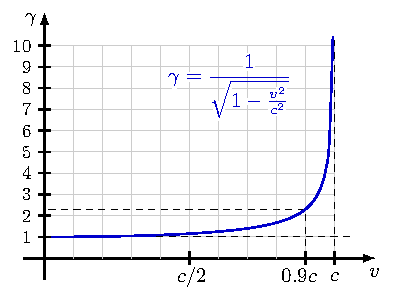
\includegraphics[width=.35\textwidth]{figures/gamma1.pdf}
\end{figure}


\begin{tcolorbox}
\begin{theorem}
\textbf{(Nokkrir eiginleikar Lorentz-fallsins)} 
\begin{enumerate}[label = \textbf{(\alph*)}]
    \item $\gamma(v) \geq 1$.
    \item $\beta = \frac{v}{c} = \sqrt{1 - \frac{1}{\gamma^2}}$
    \item $\gamma(v) \xrightarrow[v \to c]{}\ +\infty$.
    \item $\gamma(v) \approx 1 + \frac{1}{2}\left(\frac{v}{c}\right)^2$.
\end{enumerate}
\end{theorem}
\end{tcolorbox}


\section{Tímalenging}


\begin{tcolorbox}
\begin{theorem}
Lítum á lest sem ferðast með hraða $v$ miðað við athuganda $B$. Látum $A$ vera athuganda inni í lestinni. Látum ljósgjafa vera festann við gólf lestarinnar og látum spegil vera festan í lofti lestarinnar. Látum $T_A$ tákna tímann sem að athuganda $A$ sýnist það taka ljósið að endurkastast af speglinum og lenda aftur á ljósgjafanum. Látum $T_B$ tákna tímann sem að athuganda $B$ sýnist þetta sama ferli taka. Þá gildir að:
\begin{align*}
    T_B = \gamma \, T_A.
\end{align*}
\end{theorem}
\begin{figure}[H]
    \centering
    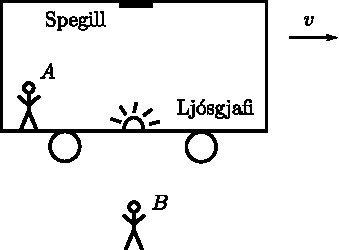
\includegraphics{figures/trains-einstein1.pdf}
\end{figure}
\end{tcolorbox}

\begin{figure}[H]
    \centering
    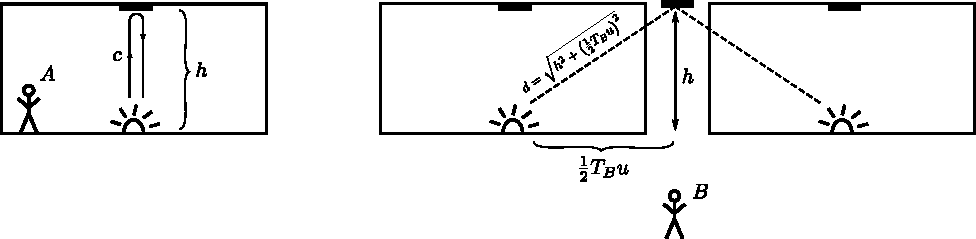
\includegraphics{figures/trains-einstein1c.pdf}
\end{figure}

\textbf{Útleiðsla:} Þá sýnist $A$ heildarvegalengdin sem ljósið þarf að ferðast vera $2h$ svo tíminn sem það tekur ljósið að ferðast þessa vegalengd er:
\begin{align*}
    T_A = \frac{2h}{c}.
\end{align*}
Hinsvegar þá sýnist $B$ ljósið þurfa að ferðast heildarvegalengdina:
\begin{align*}
    2d = 2\sqrt{h^2 + \left(\frac{1}{2}T_B v\right)^2} \implies T_B = \frac{2d}{c} = \frac{2}{c}\sqrt{h^2 + \left(\frac{1}{2}T_B v\right)^2}
\end{align*}
Við hefjum síðan í annað veldi og einangrum fyrir $T_B$. Við fáum þá að:
\begin{align*}
    T_B^2 = \frac{4}{c^2}\left(h^2 + \left(\frac{1}{2}T_B v\right)^2 \right) \implies \left(1- \left(\frac{v}{c}\right)^2 \right)T_B^2 = \frac{4h^2}{c^2} \implies T_B = \frac{\frac{2h}{c}}{\sqrt{1- \left( \frac{v}{c} \right)^2}} = \frac{T_A}{\sqrt{1- \left( \frac{v}{c} \right)^2}} = \gamma T_A.
\end{align*}
\qed


\section{Lengdarstytting}

\setcounter{theorem}{8}

\begin{tcolorbox}
\begin{minipage}{\linewidth}

\begin{wrapfigure}{r}{1.5in}
\vspace{-0.5cm}
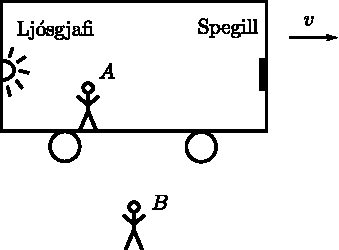
\includegraphics[width = 1.5in]{figures/trains-einstein2.pdf}
\end{wrapfigure}
\textbf{Lögmál \thetheorem.} Lítum á lest sem ferðast með hraða $v$ miðað við athuganda $B$. Látum $A$ vera athuganda inni í lestinni. Látum ljósgjafa vera festann við enda lestarinnar og látum spegil vera festan fremst í lestinni. Látum $\ell_A$ tákna lengdina sem að athuganda $A$ sýnist lestin hafa og látum $\ell_B$ tákna lengdina sem að athuganda $B$ sýnist lestin hafa. Þá gildir að:
\begin{align*}
    \ell_B = \frac{\ell_A}{\gamma}.
\end{align*}
\end{minipage}
\end{tcolorbox}

\begin{figure}[H]
    \centering
    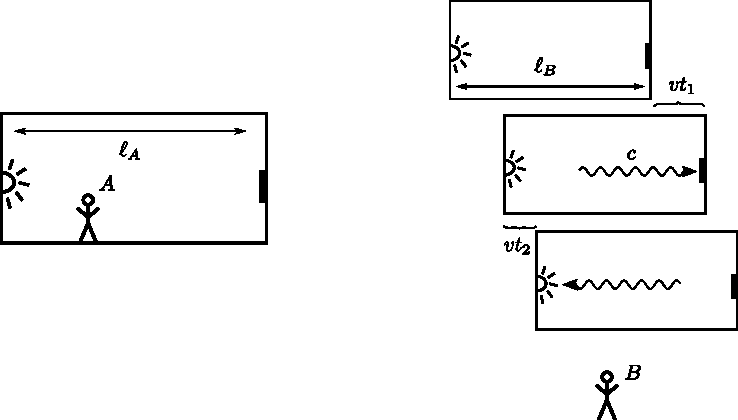
\includegraphics[scale = 0.7]{figures/trains-einstein2b.pdf}
\end{figure}

\textbf{Útleiðsla:} Tíminn sem það tekur ljósið að ferðast frá ljósgjafanum og að speglinum og aftur til baka frá sjónarhorni $A$ er gefinn með $T_A = \frac{2\ell_A}{c}$. Það sem athugandi $B$ sér er hinsvegar örlítið flóknara því lestin hreyfist á sama tíma og ljósið. Látum því $t_1$ tákna tímann sem að líður frá því að ljósið yfirgefur ljósgjafan og þar til að ljósið skellur á speglinum. Vegalengdin sem að ljósið þarf að ferðast er þá $\ell_B  + vt_1$ þannig að við fáum að:
\begin{align*}
    t_1 = \frac{\ell_B + vt_1}{c} \implies \left(1 - \frac{v}{c} \right)t_1 = \frac{\ell_B}{c} \implies t_1 = \frac{\ell_B}{c-v}.
\end{align*}
Látum síðan $t_2$ tákna tímann sem líður frá því að ljósið endurkastast af speglinum og þar til að það skellur aftur á ljósgjafanum. Þá höfum við að
Látum $t_1$ vera tímann sem það tekur ljósið að berast að speglinum og $t_2$ vera tímann sem það tekur ljósið að berast til baka í enda lestarinnar séð frá $B$. Þá gildir að:
\begin{align*}
     \ell + vt_1 = ct_1 \implies t_1 = \frac{\ell_B}{c-v}, \hspace{0.4cm} \ell - vt_2 = ct_2 \implies t_2 = \frac{\ell_B}{c+v}
\end{align*}
\begin{align*}
    t_B = t_1 + t_2 =  \frac{\ell_B}{c-v} + \frac{\ell_B}{c+v} = \frac{2\ell_B c}{c^2 - v^2} = \frac{2\ell_B}{c} \gamma^2
\end{align*}
En samkvæmt tímalengingu höfum við að $t_B = \gamma t_A$ svo:

\begin{align*}
 \gamma t_A = t_B =  \frac{2\ell_B}{c}\gamma^2 \implies t_A = \frac{2\ell_B}{c}\gamma
\end{align*}
en við vitum þegar að:
\begin{align*}
    t_A = \frac{2\ell_A}{c}
\end{align*}
en þar með er:
\begin{align*}
    \ell_A = \gamma \ell_B
\end{align*}
\qed

\section{Lorentz-ummyndanir}

\begin{tcolorbox}

\iduck{You never really understand a person until you consider things from his point of view — until you climb into his skin and walk around in it.} \\

\vspace{-0.5cm}
\raggedleft{- \textbf{Atticus Finch, To Kill a Mockingbird}}
\end{tcolorbox}

Lorentz-ummyndanir leyfa okkur að sjá veröldina með augum annarra.

\begin{tcolorbox}
\begin{theorem}
Látum $S$ og $S'$ vera tvö tregðukerfi sem hreyfast með hraða $v$ miðað við hvert annað. Látum $(x,t)$ vera atburð séð frá sjónarhorni athuganda í $S$. Þá sér athugandi í $S'$ atburðin gerast í $(x',t')$ þar sem:
\begin{align*}
    x' = \gamma (x - vt), \hspace{1cm} t' = \gamma \left( t - \frac{vx}{c^2} \right)
\end{align*}
\end{theorem}
\end{tcolorbox}

\textbf{Útleiðsla:} Hugsum okkur að athugandi í viðmiðunarkerfinu $S'$ haldi á stöng með eiginlengd $x'$. Athugandi í $S'$ mun alltaf (fyrir öll $t'$) sjá vinstri enda stangarinnar í $0$ og hægri enda stangarinnar í $x'$. Hinsvegar lítur þetta öðruvísi út fyrir athuganda í $S$. Hann sér athugandann í $S'$ fjarlægjast sig með hraða $v$ svo að stöngin mun styttast útaf lengdarstyttingu. Hann mælir því lengd stangarinnar sem $\ell = x'/\gamma$. Honum sýnist þá hægri endi stangarinnar vera staddur í $x = vt + \ell = vt + x'/\gamma$ en þá fáum við með því að leysa fyrir $x'$ að:
\begin{align*}
    x' = \gamma\left(x- vt\right).
\end{align*}
En vegna afstæðislögmálsins þá virka nákvæmlega sömu rök fyrir stöng af lengd $x$ í $S$ svo við ályktum að:
\begin{align*}
    x = \gamma \left(x' + vt' \right).
\end{align*}
En með því að einangra fyrir $t'$ úr jöfnunni hér á undan þá fáum við að:
\begin{align*}
    vt' = \frac{x}{\gamma} - x' = \frac{x}{\gamma} - \gamma \left( x - vt \right) = \gamma \left( \left( \frac{1}{\gamma^2} - 1 \right)x + vt\right) = \gamma \left( vt - \frac{v^2}{c^2}x \right).
\end{align*}
Sem gefur því að:
\begin{align*}
    t' = \gamma \left( t - \frac{v}{c^2}x \right).
\end{align*}
Með því að nota afstæðislögmálið sjáum við þá að við höfum einnig að: $t = \gamma \left( t' + \frac{v}{c^2}x \right)$.

\qed

\section{Óbreyttna tímarúmsvegalengdin}

\begin{tcolorbox}
\begin{definition}
Við segjum að stærð sé \textbf{óbreytin} ef að hún er eins í öllum viðmiðunarkerfum.
\end{definition}
\end{tcolorbox}


\begin{tcolorbox}
\begin{theorem}
Tímarúmsvegalengdin $(\Delta s)^2 = c^2 (\Delta t)^2 - (\Delta x)^2$ er óbreytin.
\end{theorem}
\end{tcolorbox}

\textbf{Útleiðsla:} Við beitum Lorentz-ummyndun á stærðina. Höfum að:
\begin{align*}
    (\Delta s')^2 &= (c\Delta t')^2 - (\Delta x')^2 \\ &= \gamma^2 \left( c \Delta t - \frac{v}{c} \Delta x \right)^2 - \gamma^2 \left( \Delta x - v\Delta t \right)^2 \\
    &= \gamma^2(c^2-v^2)(\Delta t)^2 - \gamma^2\left(1 - \frac{v^2}{c^2}\right)(\Delta x)^2 \qquad \text{(því milliliðirnir styttast út)} \\
    &= c^2 (\Delta t)^2 - (\Delta x)^2 = (\Delta s)^2.
\end{align*}
Svo við ályktum að $(\Delta s)^2$ (og þar með $\Delta s$) er óbreytin stærð því hún er eins í öllum viðmiðunarkerfum. \qed

\newpage

\section{Tímarúmsmyndir}

\begin{minipage}{\linewidth}

\begin{wrapfigure}{r}{1.75in}
\vspace{-2cm}
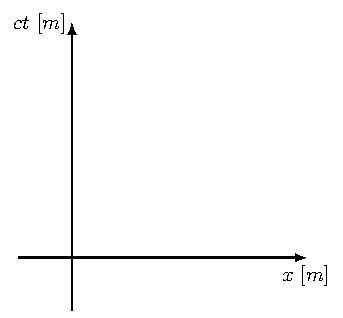
\includegraphics[width = 2.25in]{figures/spacetime1.pdf}
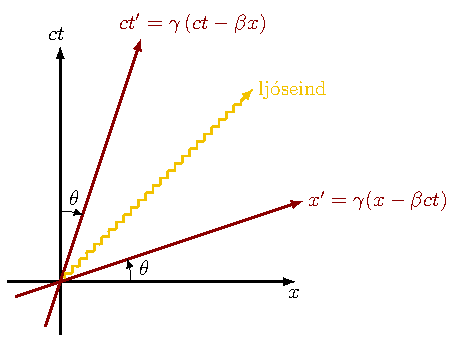
\includegraphics[width = 2.5in]{figures/spacetime2.pdf}
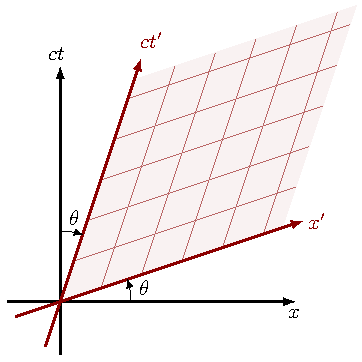
\includegraphics[width = 2.5in]{figures/spacetime3.pdf}
\end{wrapfigure}
Það getur verið gott að teikna tímarúmsmyndir í takmörkuðu afstæðiskenningunni til þess að átta sig betur á því hvað er að gerast. Við skulum í þessari grein reyna að útskýra hvernig að maður teiknar slíkar myndir og upplýsingarnar sem er hægt að lesa af þeim. Við byrjum á því að teikna tvo ása eins og sést á grafinu hér til hægri. Ástæðan fyrir því að við setjum $ct$ á lóðrétta ásinn í stað $t$ er vegna þess að $ct$ hefur sömu einingar og $x$ (þ.e.~$\si{m}$) svo þá hafa báðir ásanir sömu einingar. Það gerir líka rúmfræðina sem að við fáum út miklu fallegri að skala tímahnitið svona með $c$ (þá er reyndar oftast þægilegast að velja einingarnar á ásunum sem ljósár í staðinn fyrir metra). Þetta graf lýsir því til dæmis hvernig að athugandi í viðmiðunarkerfinu $S$ sér tímarúmið. En okkur langar til þess að bæta við hvernig athugandi í viðmiðunarkerfi $S'$ sem hreyfist afstætt með hraða $v$ miðað við $S$ sér tímarúmið. Þá bætum við inn á grafið eins og sést hér til hægri.

\vspace{0.2cm}

Hornið sem að $S'$ myndar miðað við $S$ er þá $\theta = \arctan(\beta)$ þar sem $\beta = \frac{v}{c}$ og $v$ er afstæði hraðinn milli viðmiðunarkerfanna. Við sjáum þá að þegar að $v = c$ þá verður $\theta = \arctan(\frac{c}{c}) =  \arctan(1) = \ang{45}$ sem samsvarar því sem að maður myndi sjá ef að maður væri að ferðast á ljóshraða (þá fellur tímarúmið saman í eina vídd - ljóseind upplifir þannig fjórvíða tímarúmið eins og eina vídd). Ef að við bætum við ásunum fyrir hvort hnitakerfi um sig þá getum við líka áttað okkur betur á því hvernig að upplifun athugendanna í hvoru viðmiðunarkerfi um sig breytist. Í viðmiðunarkerfinu $S'$ þá munu tveir atburðir gerast á sama tíma ef að þeir liggja á sömu línu samsíða $x'$ ásnum. Eins munu tveir atburðir gerast á sama stað ef að þeir liggja samsíða $ct'$ ásnum. Þess vegna verður hnitakerfi athugandans í $S'$ svona tígullaga séð frá $S$. Þetta tígulhnitakerfi hefur verið teiknað á myndina hér til hægri.

\vspace{0.3cm}

Skoðum núna tvo atburði $A$ og $B$. Við ætlum að reyna að skoða þá í báðum viðmiðunarkerfunum $S$ og $S'$. Til þess að gera þetta sýnidæmi áþreifanlegt skulum við láta viðmiðunarkerfin ferðast með hraða $v = \frac{1}{3}c$ miðað við hvert annað. Þá er $\beta = \frac{1}{3}$ og $\gamma = \SI{1.06}{}$ svo $\theta = \arctan(\beta) = \arctan(\frac{1}{3}) = \ang{18.4} $. Látum tímarúmshnitin á atburðunum í $S$ vera $A = (3,1) \, \si{ly}$ og $B = (2,4) \, \si{ly}$. Með Lorentz-ummyndun sjáum við að þá er:
\begin{align*}
  ct'_A = \gamma(ct_A - \beta x_A) = \SI{1.06}{} \cdot \left( 3 - \frac{1}{3} \cdot 1 \right) = \SI{2.83}{ly}.
\end{align*}
\begin{align*}
  x'_A = \gamma(x_A -  \beta ct_A) = \SI{1.06}{} \cdot \left( 1 - \frac{1}{3} \cdot 3 \right) = \SI{0}{ly}.
\end{align*}
\end{minipage}

\vspace{0.2cm}
Þannig að $A' = (\SI{2.83}{};\SI{0}{}) \, \si{ly}$. Eins fáum við að $B' = (\SI{0.71}{};\SI{3.53}{}) \, \si{ly}$ séð með augum athugandans í $S'$.

\begin{figure}[H]
    \centering
    \subfloat{{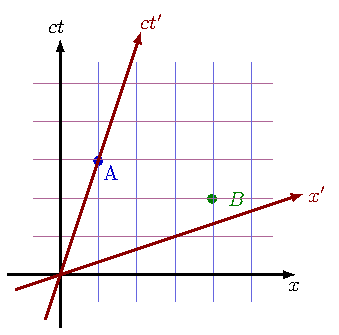
\includegraphics[scale = 0.7]{figures/spacetime5.pdf}}}%
    \qquad
    \subfloat{{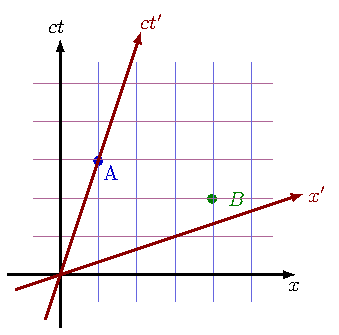
\includegraphics[scale = 0.7]{figures/spacetime5.pdf}}}%
\end{figure}

Skoðum síðan tímarúmsvegalengdina á milli punktanna $A$ og $B$ í viðmiðunarkerfunum tveimur. Í $S$ höfum við að tímarúmsvegalengdin á milli atburðanna er:
\begin{align*}
    (\Delta s)^2 = (c\Delta t)^2 - (\Delta x)^2 = (ct_B - ct_A)^2 - (x_B - x_A)^2 = (2-3)^2 - (4-1)^2 =  -\SI{8.0}{ly}.
\end{align*}
En athugandi í $S'$ mælir vegalengdina sem:
\begin{align*}
    (\Delta s')^2 = (c\Delta t')^2 - (\Delta x')^2 = (ct'_B - ct'_A)^2 - (x'_B - x'_A)^2 = (0.71-2.83)^2 - (3.53-0)^2 = -\SI{8.0}{ly}.
\end{align*}
Við sjáum semsagt að athugendurnir mæla sömu tímarúmsvegalengdina á milli atburðanna $A$ og $B$ þó að þeir séu ósammála um lengdina á milli atburðanna og tímann sem líður á milli atburðanna! Við segjum þá að tímarúmsvegalengdin sé óbreytin stærð því allir athugendur eru sammála um tímarúmsvegalengdina á milli tveggja atburða óháð viðmiðunarkerfinu þeirra. Með öðrum orðum þá er stærð óbreytin ef að hún helst óbreytt undir Lorentz-ummyndunum. Í þessu sýnidæmi þá fengum við reyndar að tímarúmsvegalengdin á milli atburðanna $A$ og $B$ var neikvæð! Má það bara? Svarið er já, það má og það hefur ákveðna merkingu sem að við skulum núna fjalla um. Tímarúmsvegalengdin getur haft þrjú formerki (er núll formerki?)

\begin{tcolorbox}
\begin{definition}
Látum $A = (x_A, t_A)$ og $B = (x_B, t_B)$ vera tvo atburði séð frá augum athuganda í viðmiðunarkerfinu $S$. Við segjum að atburðirnir $A$ og $B$ séu:
\begin{enumerate}[label = \textbf{(\roman*)}]
    \item \textbf{Tímalægir} ef $(\Delta s)^2 > 0$.
    \item \textbf{Rúmlægir} ef $(\Delta s)^2 < 0$.
    \item \textbf{Ljóslægir} ef $(\Delta s)^2 = 0$.
\end{enumerate}
\end{definition}
\end{tcolorbox}

Hvernig á maður samt að hugsa um þessi formerki? Jú, ef að $A$ og $B$ eru ljóslægir þ.e.~ef $(\Delta s)^2 = 0$ þá er eina leiðin til þess að senda skilaboð á milli atburðanna með ljósboði. Hinsvegar ef við höfum tímalæga punkta þá er $(\Delta s)^2 > 0$ en það samsvarar því að það væri hægt að ferðast á milli punktanna með hraða $v < c$. Hinsvegar ef tveir punktar eru rúmlægir þá myndi það samsvara því að eina leiðin til þess að ferðast á milli punktanna sé ef að maður ferðast með hraða $v > c$ en það er ekki hægt! Þar sem að tímarúmsvegalengdin er óbreytin þá þýðir þetta að allir athugendur eru sammála um það hvort að tveir atburðir séu tímalægir, ljóslægir eða rúmlægir. Það er annað áhugavert sem að er hægt að nefna (ég ætla ekki að leiða það hér en ef þið hafið áhuga getið þið sent mér fyrirspurn um þetta). Það kemur í ljós að ef tveir atburðir eru tímalægir þá er til viðmiðunarkerfi $S'$ þar sem að atburðirnir gerast á sama tíma. Hinsvegar ef þeir eru rúmlægir þá er til viðmiðunarkerfi $S'$ þar sem að þeir gerast í sama rúmhniti. En það er hægt að gera hvorugt fyrir ljóslæga atburði. Allar þessar niðurstöður má sjá á eftirfarandi tímarúmsmynd:
\begin{figure}[H]
    \centering
    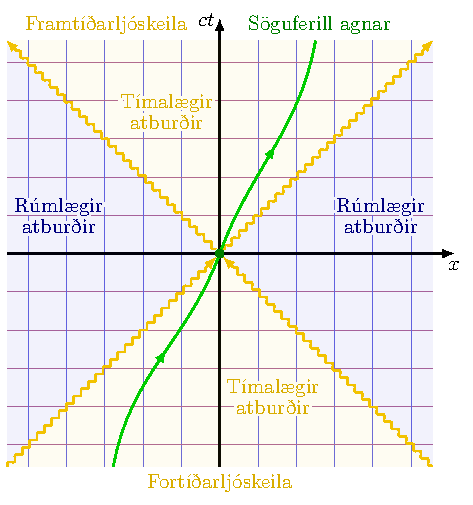
\includegraphics[scale = 0.8]{figures/spacetime6.pdf}
\end{figure}


\newpage

\section{Hraðasamlagning}

\begin{tcolorbox}
\begin{theorem}
Lítum á lest sem ferðast með hraða $v$ miðað við kyrrstæðan athuganda $B$ í viðmiðunarkerfi $S$. Látum $A$ vera athuganda inni í lestinni í viðmiðunarkerfi $S'$. Nú kastar $A$ bolta inni í lestinni með hraða $u'$. Þá sér athugandi $B$ hraða boltans sem:
\begin{align*}
    u = \frac{u' + v}{1 + \frac{vu'}{c^2}} 
\end{align*}
\end{theorem}
\end{tcolorbox}


\textbf{Útleiðsla:} Athugum fyrst að í viðmiðunarkerfinu $S'$ er staðsetning boltans $\Delta x' = u' \Delta t'$ þ.a.~við fáum:
\begin{align*}
    u = \frac{\Delta x}{\Delta t} = \frac{\gamma \left( \Delta x' + v\Delta t' \right)}{\gamma \left( \Delta t' + \frac{v}{c^2}\Delta x' \right)} = \frac{(u' + v)\Delta t'}{\left(1 + \frac{u'v}{c^2}\right)\Delta t'} = \frac{u' + v}{1 + \frac{u'v}{c^2}}.
\end{align*}
\qed

\section{Dopplerhrif fyrir ljós}

\begin{tcolorbox}
\begin{theorem}
Lítum á ljósgjafa sem sendir frá sér ljós með tíðni $f'$ í viðmiðunarkerfi ljósgjafans. Ef ljósgjafinn ferðast með hraða $v$ í áttina að kyrrstæðum athuganda þá mun athugandinn greina tíðni ljósbylgjunnar sem:
\begin{align*}
    f = \sqrt{\frac{1 + \beta}{1 - \beta}} f'
\end{align*}
\end{theorem}
\end{tcolorbox}

\begin{figure}[H]
    \centering
    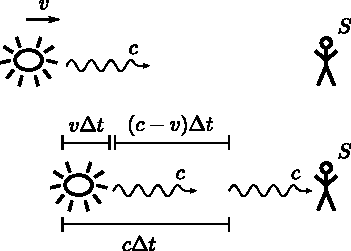
\includegraphics{figures/dopplerhrif-ljos.pdf}
\end{figure}

\textbf{Útleiðsla:} Ljósgjafinn sendir frá sér ljósbylgjur með tíðni $f'$ svo í viðmiðunarkerfi ljósgjafans líður tími $\Delta t' = \frac{1}{f'}$ á milli þess sem að ljósgjafinn sendir frá sér ljósbygljur. En athugandi í kerfinu $S$ mun sjá þetta sem lengri tíma (því tíminn í viðmiðunarkerfi ljósgjafans líður hægar því hann er á ferð) en þar með mun tíminn sem líður á milli ljósblossa vera $\Delta t = \gamma \Delta t'$ í viðmiðunarkerfi athugandans í $S$. En á þeim tíma hefur ljósgjafinn ferðast nær um vegalengd $v \Delta t$ en ljósið hefur ferðast vegalengd $c \Delta t$ svo tíminn sem líður á milli þess að athugandinn í $S$ greinir ljósblossa er:
\begin{align*}
    \Delta T = \frac{(c-v)\Delta t}{c} = \left(1 - \beta \right) \gamma \Delta t' = \frac{1-\beta}{\sqrt{1-\beta^2}}\Delta t' = \sqrt{\frac{1- \beta}{1+\beta}} \Delta t'
\end{align*}
En þar með ályktum við að tíðnin sem athugandi í $S$ greinir er gefin með:
\begin{align*}
    f = \frac{1}{\Delta T} = \sqrt{\frac{1 + \beta}{1-\beta}} \frac{1}{\Delta t'} = \sqrt{\frac{1 + \beta}{1-\beta}} f'.
\end{align*}
Sér í lagi sjáum við að $f > f'$ þegar að ljósgjafinn nálgast athugandann en $f < f'$ þegar hann fjarlægist.
\qed

\section{Skriðþungi, orka og kraftur}

\begin{tcolorbox}
\begin{definition}
\textbf{(Einstein, 1905)} Ljós með tíðni $f$ og bylgjulengd $\lambda$ hegðar sér eins og straumur agna sem við köllum \textbf{ljóseindir} þar sem hver ögn hefur orku og skriðþunga:
\begin{align*}
    E = hf = \frac{hc}{\lambda}, \hspace{1cm} p = \frac{E}{c} = \frac{h}{\lambda}.
\end{align*}
Þar sem $h = \SI{6.626e-34}{J.s}$ er fasti sem nefnist fasti Plancks.
\end{definition}
\end{tcolorbox}

\begin{tcolorbox}
\begin{theorem}
Lítum á ögn með massa $m$ sem ferðast með hraða $v$ (miðað við viðmiðunarkerfið $S$). Þá eru heildarorka og skriðþungi agnarinnar í viðmiðunarkerfinu $S$ gefnar með:
\begin{align*}
   E = \gamma mc^2, \hspace{1cm} p = \gamma mv.
\end{align*}
\end{theorem}
\end{tcolorbox}

\begin{figure}[H]
    \centering
    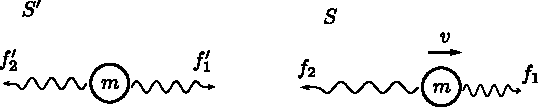
\includegraphics{figures/ljoseind-hrorna.pdf}
\end{figure}


\textbf{Útleiðsla:} Látum $S$ tákna viðmiðunarkerfi þar sem að hraði agnarinnar er $m$ og hraði hennar $v$. Látum $S'$ tákna viðmiðunarkerfi agnarinnar þar sem að ögnin er kyrr. Látum $E_0$ tákna orku eindarinnar í kyrrstöðukerfinu. Hugsum okkur nú að ögnin hrörni í tvær ljóseindir. Í kyrrstöðukerfinu þá mun önnur ljóseindin hafa tíðni $f'_1$ en hin hafa tíðni $f'_2$ en þar sem að skriðþungi kerfisins er varðveittur (miðað við kyrrstöðukerfið) er:
\begin{align*}
   0 = p'_{\text{fyrir}} = p'_1 - p'_2 \implies p'_1 = p'_2 \implies \lambda'_1 = \lambda'_2
\end{align*}
Með öðrum orðum þá hafa ljóseindirnar sömu bylgjulengd og þar með sömu tíðni í kyrrstöðukerfinu $S'$ (því þá er $f'_1 = c/\lambda'_1 = c/\lambda'_2 = f'_2$). En þar með höfum við að:
\begin{align*}
    E_0 = 2hf',
\end{align*}
þar sem $f'$ er tíðni ljóseindanna í kyrrstöðukerfinu. Skoðum næst hvað gerist í viðmiðunarkerfinu $S$ þar sem að ögnin er á hreyfingu með hraða $v$. Látum $E$ tákna orku hennar í þessu viðmiðunarkerfi og $p$ tákna skriðþunga hennar. Hugsum okkur aftur að hún hrörni í tvær ljóseindir með tíðni $f_1$ og $f_2$. Athugandi í viðmiðunarkerfinu $S$ mun greina Dopplerhrif frá ljósinu svo að:
\begin{align*}
    f_1 = \sqrt{\frac{1+\beta}{1-\beta}}f', \hspace{1cm} f_2 = \sqrt{\frac{1-\beta}{1+\beta}}f'.
\end{align*}
En þar með gildir að:
\begin{align*}
    E = hf_1 + hf_2 = hf' \left( \sqrt{\frac{1+\beta}{1-\beta}} + \sqrt{\frac{1+\beta}{1-\beta}}  \right) = hf' \frac{(1 + \beta) + (1-\beta)}{\sqrt{1-\beta^2}} = 2hf' \gamma = \gamma E_0.
\end{align*}

Svo í viðmiðunarkerfinu þar sem að ögnin er á hreyfingu þá er hreyfiorka hennar:
\begin{align*}
    K = E - E_0 = \left( \gamma -1 \right) E_0
\end{align*}
En við vitum að fyrir $v \ll c$ þ.e. $\beta \ll 1$ ættum við að endurheimta gömlu góðu hreyfiorkuna okkar, $\frac{1}{2}mv^2$, þannig að:
\begin{align*}
    K = \left( \gamma -1 \right)E_0 = \left( \left( 1 - \beta^2 \right)^{-1/2} - 1 \right) E_0 \stackrel{v \ll c}{\approx} \left(1 + \frac{\beta^2}{2} - 1 \right)E_0 = \frac{1}{2}E_0 \beta^2 \stackrel{!}{=} \frac{1}{2}mv^2
\end{align*}
En þar með sjáum við að eina leiðin til þess að $K \approx \frac{1}{2}mv^2$ er ef að $E_0 = mc^2$. Snúum okkur síðan að skriðþunganum. Þá höfum við að:
\begin{align*}
    p = \frac{h}{c} f_1 - \frac{h}{c} f_2 = \frac{hf'}{c} \left( \sqrt{\frac{1+\beta}{1-\beta}} - \sqrt{\frac{1-\beta}{1+\beta}}  \right) = \frac{hf'}{c} \frac{(1+ \beta) - (1-\beta)}{\sqrt{1-\beta^2}} = \frac{2hf'}{c} \gamma \beta
\end{align*}
En við vitum að fyrir $v \ll c$ þ.e. $\beta \ll 1$ ættum við að endurheimta gamla góða skriðþungann, $mv$, þannig að við athugum að:
\begin{align*}
    p = \frac{2hf'}{c^2}v \left(1 - \beta^2 \right)^{-1/2} \stackrel{v \ll c}{\approx} \frac{2hf' v}{c^2} \left(1 + \frac{1}{2}\left( \frac{v}{c} \right)^2 \right) \stackrel{v \ll c}{\approx} \frac{2hf' v}{c^2} \stackrel{!}{=} mv
\end{align*}
Svo við ályktum að $m = \frac{2hf'}{c^2}$. En þar með höfum við sýnt að $p = \gamma mv$.

\qed

Þetta er hin fræga niðurstaða $E = mc^2$ sem er kennd við Einstein. En í gegnum árin hefur hún skolast svolítið til. Í dag ætti maður að skrifa $E = \gamma mc^2$ en á tímum Einsteins var talað um svokallaðan kyrrstöðu massa $m_0$ og massi hlutarins var þá $m(v) = \gamma m_0$. En það er frekar óheppilegt ef að massi hluta breytist eftir viðmiðunarkerfum. Það er þægilegra að tala um að hinn svokallaði kyrrstöðumassi sé massi hlutarins (annars þarf maður líka að fara að tala um svokallaðan þvermassa og langsmassa og massinn er þá mismikill í mismunandi stefnur sem er algjör hausverkur).


\begin{tcolorbox}
\begin{definition}
Stærðin $E_0 = U = mc^2$ kallast \textbf{kyrrstöðuorka} massans $m$ og er óbreytin stærð.
\end{definition}
\end{tcolorbox}

\begin{tcolorbox}
\begin{definition}
    Stærðin $K = (\gamma -1)mc^2$ kallast \textbf{hreyfiorka} massans $m$.
\end{definition}
\end{tcolorbox}
Við sjáum þá sér í lagi að $K + U = K + E_0 = \gamma mc^2 = E$ er heildarorka massans $m$.

\begin{tcolorbox}
\begin{theorem}
Látum $E$ og $p$ tákna heildarorku og skriðþunga eindar í viðmiðunarkerfinu $S$. Þá er stærðin $E^2 - (pc)^2$ óbreytin og sér í lagi gildir að:
\begin{align*}
E^2 - (pc)^2 = E_0^2 = (E')^2 - (p'c)^2
\end{align*}
Þar sem $E'$ og $p'$ eru heildarorka og skriðþungi eindarinnar í viðmiðunarkerfinu $S'$.
\end{theorem}
\end{tcolorbox}

\textbf{Útleiðsla:} Þetta er bara einföld algebruæfing. Athugum fyrst að $pc = \gamma mvc = \gamma \beta mc^2$. Fáum því að:
\begin{align*}
    E^2 - (pc)^2 = \left(\gamma mc^2 \right)^2 - (\gamma \beta mc^2)^2 = \gamma^2 \left( 1 - \beta^2\right)(mc^2)^2 = (mc^2)^2 = E_0^2
\end{align*}
Sem er óbreytin stærð svo þar með höfum við sýnt að $E^2 - (pc)^2$ sé einnig óbreytin. \\ \qed

Mikilvægasta lögmál eðlisfræðinnar er kennt við stærðfræðinginn, Emmy Noether, og útskýrir tengslin á milli samhverfu og varðveislulögmálanna. Í klassískri eðlisfræði staðhæfir lögmál Noethers að orka er varðveitt ef að heildarorka kerfisins er óbreytt undir vörpuninni $t \to t + \Delta t$ (með öðrum orðum að það skipti ekki máli hvernig að við skilgreinum upphafstímann). Eins má sýna með lögmáli Noethers að skriðþungi kerfisins er varðveittur ef að heildarorka kerfisins er óbreytt undir vörpuninni $x \to x + \Delta x$ (með öðrum orðum ef að það skiptir ekki máli hvar við skilgreinum upphafspunktinn). Að lokum fáum við hverfiþungavarðveislu samkvæmt lögmálum Noethers ef að heildarorka kerfisins er óbreytin undir snúningum $\Vec{r} \to \Vec{r}'$ (með öðrum orðum að það skiptir ekki máli hvernig að við skilgreinum upphafshornið).

\newpage


\section{Nálganir}

Í þessum undirkafla ætlum við að sýna að ef að við gerum þá nálgun að $v \ll c$ þá endurheimtum við gömlu góðu klassísku eðlisfræðina okkar. Þar með erum við að sýna að takmarkaða afstæðiskenningin inniheldur alla þá eðlisfræði sem að við þekkjum og gott betur! Í rauninni byggja allar nálganirnar í þessari undirgrein á uppáhalds nálgun eðlisfræðingsins:
\begin{align*}
    (1 + x)^n \approx 1 + nx, \hspace{1cm} \text{ef $\abs{x} \ll 1$}.
\end{align*}
Við byrjum á því að skoða lengdarstyttinguna:
\begin{align*}
    \ell = \frac{\ell_0}{\gamma} = \ell_0 \sqrt{1 - \frac{v^2}{c^2}} = \ell_0 \left( 1 - \frac{v^2}{c^2} \right)^{1/2} \explain{\approx}{\frac{v^2}{c^2} \ll 1} \ell_0 \left( 1 - \frac{1}{2} \frac{v^2}{c^2} \right) = \ell_0 - \frac{1}{2}\ell_0 \frac{v^2}{c^2}. 
\end{align*}
Svo í fyrstu Taylor-nálgun þá sjáum við að $\ell \approx \ell_0$ (ef $\frac{v^2}{c^2} \ll 1$). Skoðum síðan næst tímalenginguna:
\begin{align*}
    t = \gamma t_0 = \frac{t_0}{\sqrt{1 - \frac{v^2}{c^2}}} = t_0\left( 1 - \frac{v^2}{c^2} \right)^{-1/2} \approx t_0 \left( 1  + \frac{1}{2} \frac{v^2}{c^2}  \right) = t_0 + \frac{1}{2}t_0 \frac{v^2}{c^2}. 
\end{align*}
Svo við sjáum aftur í fyrstu nálgun að $t \approx t_0$ (ef $\frac{v^2}{c^2} \ll 1$). Skoðum síðan Lorentz-ummyndanirnar:
\begin{align*}
    x' = \gamma \left( x - vt \right) = \left( x - vt \right)\left(1 - \frac{v^2}{c^2} \right)^{-1/2} \approx \left( x - vt \right)\left(1 + \frac{1}{2}\frac{v^2}{c^2} \right) \approx x- vt.
\end{align*}
Eins fæst fyrir tímann að:
\begin{align*}
    t' = \gamma \left( t - \frac{v}{c^2}x \right) \approx \left(t - \frac{v}{c^2}x \right)\left( 1 + \frac{1}{2}\frac{v^2}{c^2} \right) \approx t
\end{align*}
Við sjáum því að við fáum $t' = t$ og $x' = x- vt$ sem að eru einmitt Galíleó-ummyndanirnar. Skoðum næst hraðasamlagninguna:

\begin{align*}
    u' = \frac{u-v}{1 - \frac{uv}{c^2}} = (u-v)\left(1 - \frac{uv}{c^2} \right)^{-1} \approx (u-v)\left(1 + \frac{uv}{c^2} \right) \approx (u-v).
\end{align*}
Fyrir Dopplerhrifin fáum við:
\begin{align*}
    f = \left(1 + \beta \right)^{1/2}\left(1 - \beta \right)^{-1/2} f' \approx \left(1 + \frac{\beta}{2} \right) \left(1 + \frac{\beta}{2} \right)f' \approx f' + \beta f' = (1+\beta)f' = \left(1 + \frac{v}{c} \right)f'
\end{align*}
Sem er einmitt það sem að við myndum búast við í klassískri eðlisfræði. Loks er:
\begin{align*}
    E = \gamma mc^2 \approx mc^2 \left(1 + \frac{1}{2}\frac{v^2}{c^2} \right) = mc^2 + \frac{1}{2}mv^2.
\end{align*}
og þá sér í lagi $K = (\gamma -1)mc^2 \approx \frac{1}{2}mv^2$ og loks höfum við að:
\begin{align*}
    p = \gamma mv \approx mv\left(1 - \frac{1}{2}\frac{v^2}{c^2} \right) \approx mv.
\end{align*}
Við höfum semsagt sýnt að í öllum tilvikum endurheimtum við klassísku eðlisfræðina okkar.


\newpage

\section{Dæmi}

\subsection*{Dæmatími 31: Afstæðiskenningin: Tímaþennsla}

\begin{tcolorbox}
Ljóshraðinn, $c$, er sá sami í öllum tregðukerfum. Ef $t_0$ er tíminn og $\ell_0$ er lengdin sem að athugandi mælir í lest sem ferðast með hraða $v$. Þá er tíminn og lengdin sem að kyrrstæður athugandi á brautarpallinum mælir:
\begin{align*}
    t = \gamma t_0, \hspace{1cm} \ell = \frac{\ell_0}{\gamma}, \hspace{1cm} \text{þar sem} \hspace{0.5cm} \gamma = \frac{1}{\sqrt{1-\left(\frac{v}{c}\right)^2}}.
\end{align*}
\end{tcolorbox}

\begin{enumerate}[label = \textbf{(\alph*)}]


\item[\textbf{(36.13)}] Athugandi á jörðinni sér mýeind ferðast \SI{60}{km} vegalengd í lofthjúp jarðar á \SI{400}{\mu s}. Hvað tekur þetta langan tíma samkvæmt mýeindinni?

\item[\textbf{(36.15)}] Geimfari nokkur hefur verið sendur með geimflaug í áttina að Proxima Centauri, sem er sú stjarna sem er næst sólinni okkar. Hún er í \SI{4.24}{} ljósára fjarlægð og geimflaugin ferðast með hraðanum $0,80c$.
\begin{enumerate*}[label = \textbf{(\alph*)}]
    \item Hversu langan tíma tekur ferðin samkvæmt jarðarbúum?
    \item Hversu langan tíma tekur ferðin samkvæmt geimfaranum?
    \item Þegar geimfarinn nær til Proxima Centauri sendir hann útvarpsboð til baka til jarðarinnar. Hversu löngu eftir að geimfarinn lagði af stað munu jarðarbúar heyra skilaboðin?
\end{enumerate*}

\item[\textbf{(36.16)}] Elon Musk hefur séð fram á það að hann muni ekki ná að sjá næstu þvergöngu Venusar árið 2117 þar eð hann verður ellidauður. En Elon Musk dettur það snilldarráð í hug að stökkva upp í SpaceX geimflaugina sína og fljúga með hraða $v$ (miðað við viðmiðunarkerfi jarðarinnar) í áttina að nálægri fjarreikistjörnu og snúa þar við og koma síðan aftur til jarðarinnar. Hann ætlar að skipuleggja ferðina þannig að hann eldist sjálfur aðeins um \SI{5}{ár} á meðan að athugendur á jörðinni eldast um \SI{90}{ár}. \begin{enumerate*}[label = \textbf{(\alph*)}]
    \item Hver þarf hraði geimflaugarinnar, $v$, að vera?
    \item Hversu langt er til fjarreikistjörnunnar?
\end{enumerate*}

\item[\textbf{(36.19)}] Mark Cuban á lífstíðarflugpassa með American Airlines sem þýðir að hann býður stundum Dirk Nowitzki frítt flug heim til Berlínar frá Dallas. Flugvegalengdin er um það bil \SI{8550}{km} og flugvélin ferðast með hraða \SI{900}{km/klst}. Hversu mikið yngjast Cuban og Nowitzki miðað við fólkið í Dallas á því að fljúga svona fram og tilbaka? (\textit{Ábending:} Þið gætuð þurft að nota nálgunina $(1+x)^n \approx 1+ nx$).

\end{enumerate}

\begin{tcolorbox}
\begin{enumerate*}[label = ]
  \item \textbf{(36.13)} $\SI{350}{\mu s}$.
  \item \textbf{(36.15)} $\SI{5,3}{ár}$, $\SI{3,2}{ár}$, $\SI{9,5}{ár}$.
  \item \textbf{(36.16)} $0,998c$, $\SI{44,9}{ly}$
  \item \textbf{(36.19)} $\SI{11.9}{ns}$.
\end{enumerate*}
\end{tcolorbox}

\newpage

\subsection*{Dæmatími 32: Afstæðiskenningin: Lengdarstytting}

\begin{tcolorbox}
Ljóshraðinn, $c$, er sá sami í öllum tregðukerfum. Ef $t_0$ er tíminn og $\ell_0$ er lengdin sem að athugandi mælir í lest sem ferðast með hraða $v$. Þá er tíminn og lengdin sem að kyrrstæður athugandi á brautarpallinum mælir:
\begin{align*}
    t = \gamma t_0, \hspace{1cm} \ell = \frac{\ell_0}{\gamma}, \hspace{1cm} \text{þar sem} \hspace{0.5cm} \gamma = \frac{1}{\sqrt{1-\left(\frac{v}{c}\right)^2}}.
\end{align*}
\end{tcolorbox}

\begin{enumerate}[label = \textbf{(\alph*)}]

\begin{minipage}{\linewidth}

\begin{wrapfigure}{r}{1.75in}
\vspace{-0.5cm}
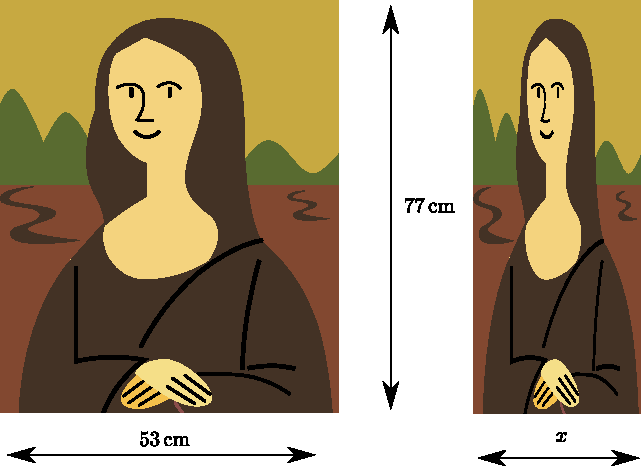
\includegraphics[width = 2.25in]{figures/mona-lisa.pdf}
\end{wrapfigure}

\item[\textbf{(36.20)}] Móna Lísa er frægt olíumálverk eftir Leonardo da Vinci sem er til sýnis á Louvre-safninu í París. Málverkið er aðeins $\SI{77}{cm}$ á hæð og $\SI{55}{cm}$ á breidd. Nýlega hafa frönsk stjórnvöld farið að bjóða geimferðamönnum að fljúga í gegnum safnið á ógnarhraða, $0,90c$, til þess að bera málverkið augum án þess að þurfa að bíða í röðinni með jarðarbúum. Hversu breitt sýnist þeim þá málverkið vera?

\item[\textbf{(36.23)}] Mýeind ferðast í gegnum lofthjúp jarðar með hraðanum $0,9997c$ miðað við athuganda á jörðinni. Frá athugandanum séð þá ferðast mýeindin \SI{60}{km} vegalengd frá því að hún myndaðist og þar til að hún hrörnaði. \begin{enumerate*}[label = \textbf{(\alph*)}]
    \item Hver er líftími mýeindarinnar séð frá sjónarhóli athugandans á jörðinni?
    \item Hversu langa vegalengd finnst mýeindin eins og að hún hafi ferðast?
    \item Hver er líftími mýeindarinnar frá hennar eigin sjónarhorni?
\end{enumerate*}

\item[\textbf{(36.21)}] Með hvaða hraða þarf stöng að ferðast til þess að hún líti út fyrir að vera helmingi styttri en hún er?

\item[\textbf{(36.25)}] Mannshár er um það bil \SI{50}{\mu m} í þvermál. Gregor Clegane á \SI{143}{cm} langt sverð. Hann þrumar sverðinu sínu í áttina að Oberyn Martell sem rétt nær að víkja undan sverðinu. Þegar að sverðið ferðast framhjá Oberyn sýnist honum sverðið ekki vera lengra heldur en mannshár. Hver var hraði sverðsins?  (\textit{Ábending:} Þið gætuð þurft að nota nálgunina $(1+x)^n \approx 1+ nx$).

\end{minipage}


\end{enumerate}

\begin{tcolorbox}
\begin{enumerate*}[label = ]
  \item \textbf{(36.20)} $\SI{23}{cm}$.
  \item \textbf{(36.23)} $\SI{200}{\mu s}$, $\SI{1.5}{km}$, $\SI{4.9}{\mu s}$.
  \item \textbf{(36.21)} $0,866c$.
  \item \textbf{(36.25)} $0,9999999994c$.
\end{enumerate*}
\end{tcolorbox}

\newpage

\subsection*{Dæmatími 33: Afstæðiskenningin: Hraðasamlagning og Lorentz-ummyndanir}

\begin{tcolorbox}
Ef að atburður gerist í tímarúmspunktinum $(x,t)$ í viðmiðunarkerfinu $S$ þá sér $S'$ atburðin gerast í:
\begin{align*}
    \Delta x' = \gamma \left( \Delta x - v\Delta t \right), \hspace{1cm} \Delta t' = \gamma \left( \Delta t - \frac{v\Delta x}{c^2} \right).
\end{align*}
Ef að athugandi í $S'$ kastar bolta með hraða $u'$ þá sér athugandi í $S$ boltan hafa hraða $u$ þar sem:
\begin{align*}
    u = \frac{u' + v}{1 + \frac{u' v}{c^2}}, \hspace{0.75cm} \text{sem má líka snúa við með afstæðislögmálinu:} \hspace{0.75cm} u' = \frac{u-v}{1 - \frac{uv}{c^2}}. 
\end{align*}
\end{tcolorbox}

\begin{enumerate}[label = \textbf{(\alph*)}]

\item[\textbf{(36.31)}] Matti Svifdal keyrir í DeLorean kagga með hraða $0,60c$ beint í áttina að klikkaða vísindamanninum Doksa sem ferðast beint í áttina að Matta í risastórri járnbrautalest með hraða $0,80c$. Með hvaða hraða sýnist Matta að Doksi nálgist hann?

\begin{comment}
\item[\textbf{(36.29)}] Hans Óli þýtur framhjá jörðinni með hraðanum $0,80c$ á geimskutlunni sinni, Þúsaldarfálkanum. Loðinbarði förunautur hans skýtur byssukúlu út um afturenda geimflaugarinnar með hraða $0,90c$ miðað við geimflaugina. Hver er hraði byssukúlunnar séð frá jörðinni?
\end{comment}

\item[\textbf{(36.55)}] Hans Óli og förunautur hans Loðinbarði þjóta framhjá Naboo með hraðanum $0,80c$ á geimskutlunni sinni, Þúsaldarfálkanum (sem hefur raunverulega lengd \SI{35}{m}). Logi Geimgengill flýgur í áttina að félögum sínum á X-vængnum, Rauðu fimmunni, með hraðanum $0,60c$.
\begin{enumerate*}[label = \textbf{(\alph*)}]
    \item Hversu langur sýnist Loga Þúsaldarfálkinn vera?
    \item Nú nálgast Svarthöfði óðfluga hetjurnar í Þúsaldarfálkanum með hraðanum $0,90c$ svo Loðinbarði skýtur byssukúlu út um afurenda geimflaugarinnar með hraða $0,95c$ miðað við geimflaugina þeirra. Með hvaða hraða sér Svarthöfði byssukúluna nálgast sig?
\end{enumerate*}

\item[\textbf{(36.53.)}] Matti og Edda horfa á sprengistjörnuna Delta ($D$) springa í geimsjónaukanum hans Matta. Þau sjá líka fyrir tilviljun þrjú geimskip af geimverum flýja frá sólkerfi sprengistjörnunnar Delta í áttina að stjöruninni Epsilon ($E$). Geimskip geimveranna ferðast með hraða $v_1 = 0,30c$, $v_2 = 0,50c$ og $v_3 = 0,70c$ og stjarnan Epsilon er í \SI{2}{ljósára} fjarlægð frá Delta (frá sjónarhóli Matta og Eddu). Einu ári síðar þá sjá Matti og Edda hinsvegar fyrirheitnu stjörnuna, Epsilon, springa í loft upp. Allir athugendurnir velja upphafspunkt tímarúmsins þannig að Delta springur í $(0,0)$.
\begin{enumerate*}[label = \textbf{(\alph*)}]
    \item Hvenær springur sprengistjarnan Epsilon í viðmiðunarkerfum athugendanna í geimskipunum þremur?
    \item Er einhver athugandi í viðmiðunarkerfi þar sem að sprengingarnar gerast á sama tíma?
    \item Er einhver athugandi í viðmiðunarkerfi þar sem að Epsilon springur á undan Delta?
    \item Eru sprengingarnar tímalægir ($(\Delta s)^2 > 0$), rúmlægir ($(\Delta s)^2 < 0$) eða ljóslægir atburðir ($(\Delta s)^2 = 0$)?
\end{enumerate*}

\item[\textbf{(36.74)}] Tvö geimskip hafa raunverulega lengd \SI{1000}{m} (miðað við sitt eigið viðmiðunarkerfi). Anna, kapteininn á geimskipi $A$ er að taka fram úr Baldri, kapteininum á geimskipi $B$. Anna flýgur skipinu sínu með hraða $0,80c$ en Baldur sniglast áfram á $0,60c$ (bæði er miðað við það sem áhorfandi á jörðinni sér). Hversu langan tíma finnst Baldri það taka Önnu að taka fram úr sér? Tímatakan hefst þegar að fremri endinn á geimskipi Önnu nemur við afturendan á geimskipi Baldurs og stöðvast þegar afturendinn á geimskipi Önnu yfirgefur framendan á geimskipi Baldurs.

\end{enumerate}

\begin{tcolorbox}
\begin{enumerate*}[label = ]
  \item \textbf{(36.31)} $0,95c$.
  \item \textbf{(36.55)} $\SI{10.9}{m}$, $0,976c$.
  \item \textbf{(36.53)} $(t_1,x_1) = (\SI{0.42}{ár}, \SI{1.78}{ly})$,  $(t_2,x_2) = (\SI{0}{ár}, \SI{1.73}{ly})$, $(t_3,x_3) = (-\SI{0.56}{ár}, \SI{1.82}{ly})$.
  \item \textbf{(36.74)} $\SI{16.6}{\mu s}$.
\end{enumerate*}
\end{tcolorbox}

\newpage

\subsection*{Dæmatími 34: Afstæðiskenningin: Orka og skriðþungi}

\begin{tcolorbox}
Heildarorka, skriðþungi, kyrrstöðuorka og hreyfiorka einda eru gefnar með:
\begin{align*}
    E = \gamma mc^2, \hspace{1cm} p = \gamma mv, \hspace{1cm} E_0 = mc^2, \hspace{1cm} K = E-E_0 = (\gamma -1)mc^2.
\end{align*}
Sér í lagi gildir að:
\begin{align*}
    E^2 - (pc)^2 = E_0^2
\end{align*}
Ljóseindir hafa skammtaða orku sem er háð tíðni ljóssins: $E = hf = \frac{hc}{\lambda}$ þar sem $h = \SI{6.626e-34}{J.s}$ er fasti sem kallast fasti Plancks. Ljóseindir eru massalausar svo sér í lagi gildir um þær að $E = pc$.
\end{tcolorbox}

\begin{enumerate}[label = \textbf{(\alph*)}]

\item[\textbf{(36.39)}] \begin{enumerate}[label = \textbf{(\alph*)}]
    \item Við hvaða hraða er skriðþungi eindar tvisvar sinnum meiri heldur en klassíski skriðþunginn?
    \item Við hvaða hraða er heildarorka eindar tvisvar sinnum meiri heldur en kyrrstöðuorka hennar?
    \item Við hvaða hraða er hreyfiorka eindar tvisvar sinnum meiri heldur en kyrrstöðuorka hennar?
    \begin{comment}
    \item Við hvaða hraða er hreyfiorka eindar tvisvar sinnum meiri heldur en klassíska hreyfiorkan?
    \end{comment}
\end{enumerate}

\item[\textbf{(37.26)}] Rafeindarvoltið ($\si{eV}$) er mælieining á orku sem er mikið notuð í kjarneðlis- og öreindafræði. Einingin er skilgreind sem sú orka sem að rafeind fær við það að vera hraðað yfir \SI{1}{V} spennumun en þá gildir að: $\SI{1}{eV} = \SI{1.602e-19}{J}$.
\begin{enumerate*}[label = \textbf{(\alph*)}]
    \item Hver er kyrrstöðurorka rafeindar í \si{eV}? En róteindar?
    \item Hver er heildarorka rafeindar sem að ferðast með hraðanum $0,99c$? En róteindar?
    \item Hver er hraði rafeindar sem að hefur heildarorku \SI{2.0}{GeV}? En róteindar?
\end{enumerate*}

\item[\textbf{(36.73)}] Rafeind ferðast með hraða $0,90c$ í áttina að jáeind sem hefur hraða $0,90c$ í gagnstæða stefnu. Í árekstrinum eyðast báðar eindirnar og orkan sem losnar í árekstrinum fer í að mynda tvær eins ljóseindir. Hver er bylgjulengd ljóseindanna?

\item[\textbf{(37.28)}] Í stóra sterkeindahraðalinum LHC (Large Hadron Collider) í Genf, Sviss eru róteindir með heildarorku \SI{6.5}{TeV} látnar lenda í árekstri við hvor aðra. \begin{enumerate*}[label = \textbf{(\alph*)}]
    \item Hver er hraði eindanna?
    \item Í slíkum árekstrum myndast oft ótalmargar orkuríkar öreindir. Fræðilega séð (það er mjög ólíklegt) getur myndast ein gríðarlega orkurík öreind (slík öreind væri óstöðug og myndi fljótlega hrörna niður í aðrar öreindir) í árekstrinum. Hver væri massi eindarinnar?
\end{enumerate*} 

\end{enumerate}

\begin{tcolorbox}
\begin{enumerate*}[label = ]
  \item \textbf{(36.39)} $v_a = 0,866c$, $v_b = 0,866c$, $v_c = 0,943c$.
  \item \textbf{(37.26)} $E_{0,e} = \SI{0.511}{MeV}$, $E_{0,p} = \SI{938.3}{MeV}$, $E_e = \SI{3.62}{MeV}$, $E_p = \SI{6652}{MeV}$, $v_e = 0,99999997c$, $v_p = 0,883c$.
  \item \textbf{(36.73)} $\SI{1.06}{pm}$. \\
  \item \textbf{(37.28)} $\SI{1.26e-26}{kg}$.
\end{enumerate*}
\end{tcolorbox}

\newpage